\documentclass[tikz,border=2mm]{standalone}
\usepackage[T1]{fontenc}
\usepackage{lmodern}
\usetikzlibrary{arrows.meta,positioning,fit,calc}

\definecolor{inputfill}{HTML}{DCEAF7}
\definecolor{llmfill}{HTML}{E9E0F4}
\definecolor{rulefill}{HTML}{F5E0B8}
\definecolor{evalfill}{HTML}{E2F0DC}
\definecolor{diagfill}{HTML}{F2D6D6}

\begin{document}
\sffamily
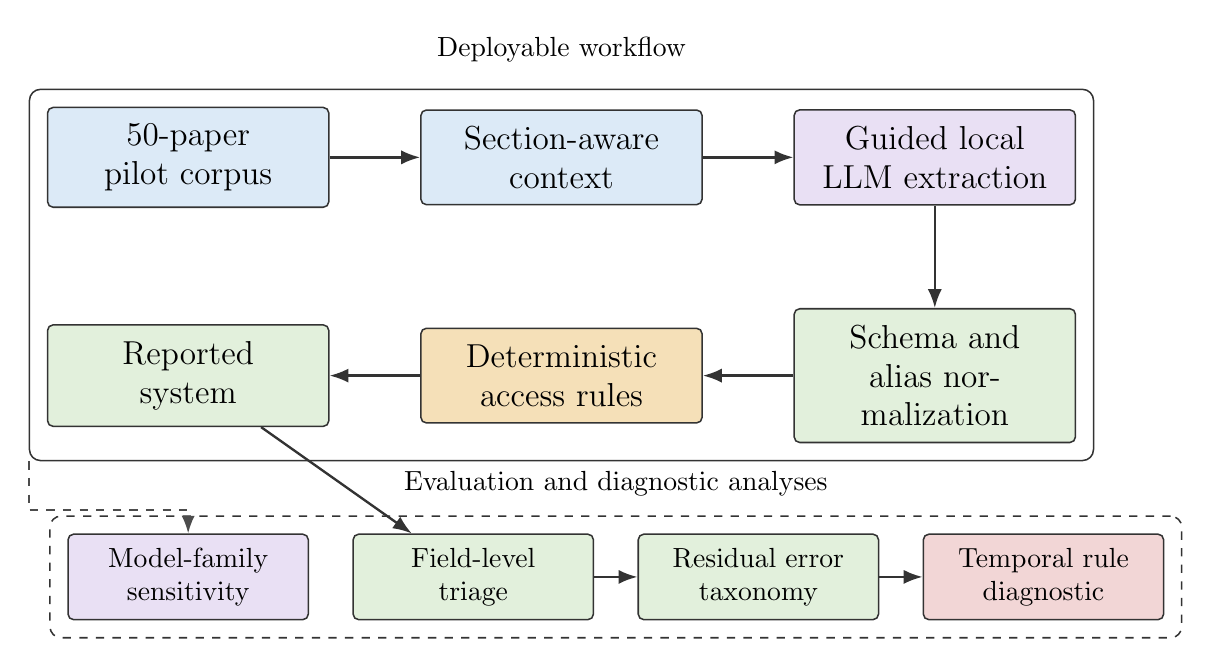
\begin{tikzpicture}[
  >=Latex,
  line/.style={draw=black!80, line width=0.55pt},
  arrow/.style={-Latex, draw=black!80, line width=0.85pt},
  box/.style={line, rounded corners=2pt, minimum height=1.10cm, text width=3.15cm, align=center, inner sep=6pt, font=\large},
  smallbox/.style={line, rounded corners=2pt, minimum height=0.95cm, text width=2.70cm, align=center, inner sep=5pt, font=\normalsize},
  note/.style={align=center, font=\normalsize},
  dashedarrow/.style={-Latex, draw=black!70, line width=0.75pt, dashed}
]

\node[box, fill=inputfill] (corpus) {50-paper\\pilot corpus};
\node[box, fill=inputfill, right=1.15cm of corpus] (context) {Section-aware\\context};
\node[box, fill=llmfill, right=1.15cm of context] (llm) {Guided local\\LLM extraction};
\node[box, fill=evalfill, below=1.30cm of llm] (norm) {Schema and\\alias normalization};
\node[box, fill=rulefill, left=1.15cm of norm] (access) {Deterministic\\access rules};
\node[box, fill=evalfill, left=1.15cm of access] (system) {Reported\\system};

\draw[arrow] (corpus) -- (context);
\draw[arrow] (context) -- (llm);
\draw[arrow] (llm) -- (norm);
\draw[arrow] (norm) -- (access);
\draw[arrow] (access) -- (system);

\node[smallbox, fill=llmfill, below=1.35cm of system] (models) {Model-family\\sensitivity};
\node[smallbox, fill=evalfill, right=0.55cm of models] (triage) {Field-level\\triage};
\node[smallbox, fill=evalfill, right=0.55cm of triage] (errors) {Residual error\\taxonomy};
\node[smallbox, fill=diagfill, right=0.55cm of errors] (temporal) {Temporal rule\\diagnostic};

\node[line, rounded corners=4pt, fit=(corpus)(context)(llm)(norm)(access)(system), inner sep=0.22cm] (mainfit) {};
\node[note, above=0.22cm of mainfit.north] {Deployable workflow};
\node[line, rounded corners=4pt, dashed, fit=(models)(triage)(errors)(temporal), inner sep=0.22cm] (evalfit) {};
\node[note, above=0.12cm of evalfit.north] {Evaluation and diagnostic analyses};

\draw[arrow] (system) -- (triage);
\draw[arrow] (triage) -- (errors);
\draw[arrow] (errors) -- (temporal);
\draw[dashedarrow] (mainfit.south west) -- ++(0,-0.62) -| (models.north);

\end{tikzpicture}
\end{document}
